%!TEX root = ../Grunddatei.tex
\section{Anhang}

\begin{figure}[ht]
    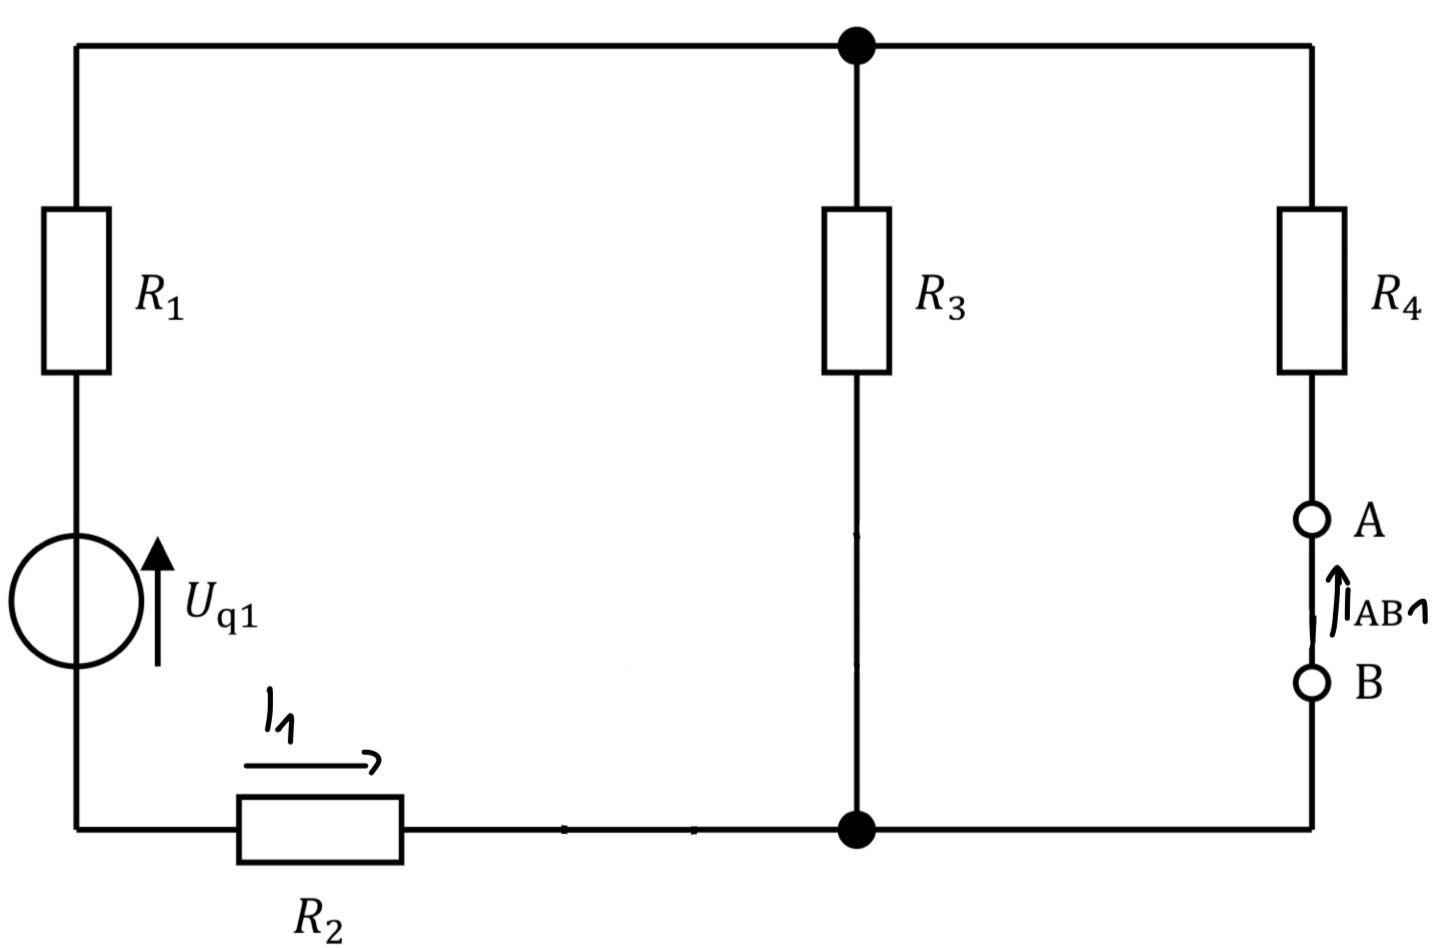
\includegraphics[width=0.6\linewidth]{Bilder/Helmholtz1.png}
    \caption{Kurzschalten von $U_2$ und $U_3$}
    \label{fig:helmholtz1}
\end{figure}
\begin{figure}[ht]
    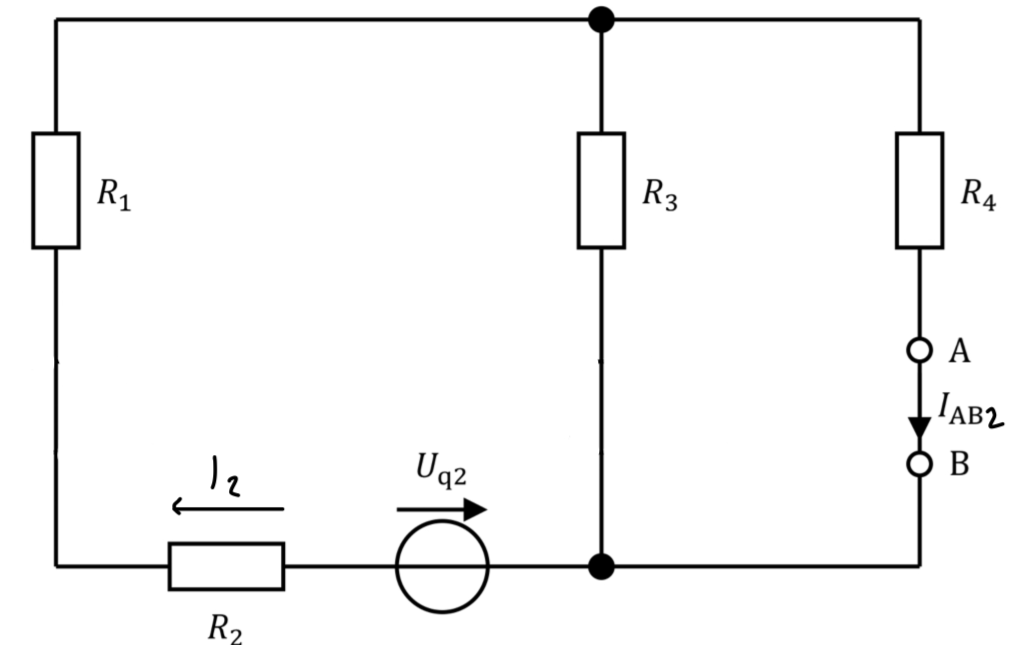
\includegraphics[width=0.6\linewidth]{Bilder/Helmholtz2.png}
    \caption{Kurzschalten von $U_1$ und $U_3$}
    \label{fig:helmholtz2}
\end{figure}
\begin{figure}[t]
    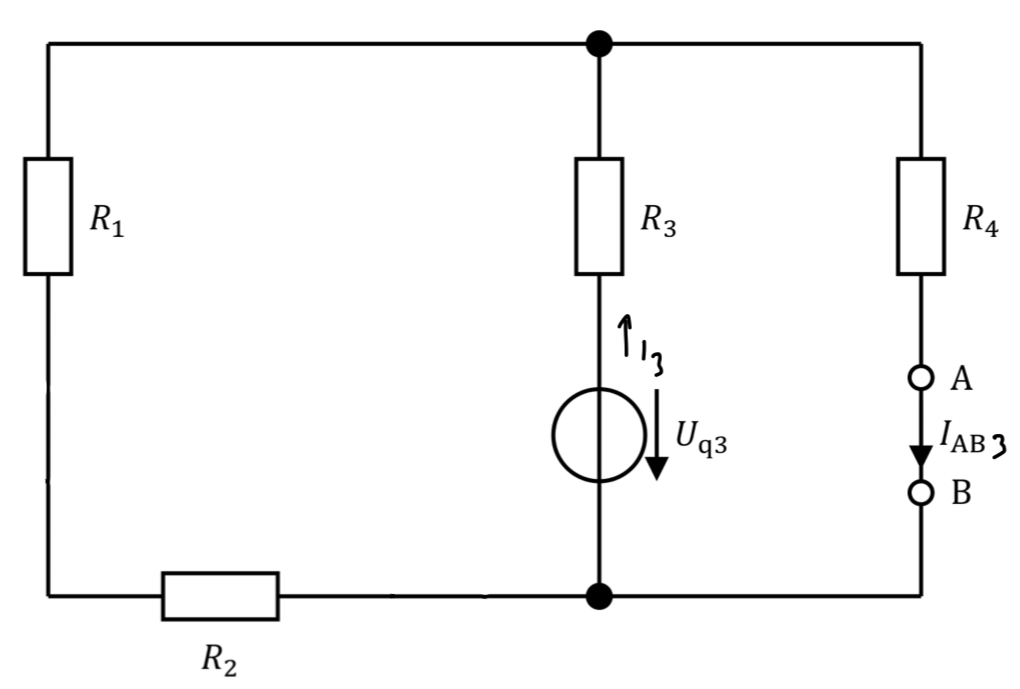
\includegraphics[width=0.6\linewidth]{Bilder/Helmholtz3.png}
    \caption{Kurzschalten von $U_1$ und $U_2$}
    \label{fig:helmholtz3}
\end{figure}
